\begin{flushright} {\tiny {\color{gray} (tikz\_globaljump.tex)}} \end{flushright}
%~~~~~~~~~~~~~~~~~~~~~~~~~~~~~~~~~~~~~~~~~~~~~~~~~~~~~~~~~~~~~~~~~~~~~~~~~~~~~~~~~~~~~~~~~~~~~~~~~~

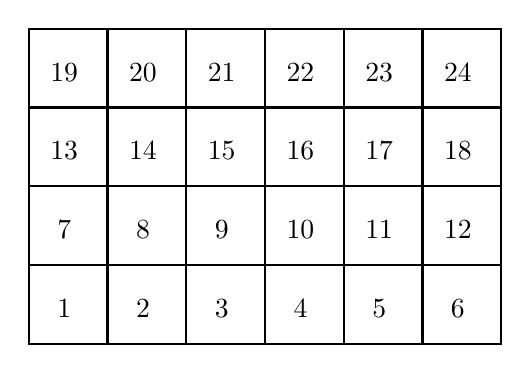
\begin{tikzpicture}
%\draw[step=0.5cm,gray,very thin] (0,0) grid (6,4); %background grid

\draw[thick] (0,0)--(6,0)--(6,4)--(0,4)--cycle;  

\draw[thick] (0,1)--(6,1);  
\draw[thick] (0,2)--(6,2);  
\draw[thick] (0,3)--(6,3);  

\draw[thick] (1,0)--(1,4);  
\draw[thick] (2,0)--(2,4);  
\draw[thick] (3,0)--(3,4);  
\draw[thick] (4,0)--(4,4);  
\draw[thick] (5,0)--(5,4);  

\node[] at (0.45,0.45) {1};
\node[] at (1.45,0.45) {2};
\node[] at (2.45,0.45) {3};
\node[] at (3.45,0.45) {4};
\node[] at (4.45,0.45) {5};
\node[] at (5.45,0.45) {6};

\node[] at (0.45,1.45) {7};
\node[] at (1.45,1.45) {8};
\node[] at (2.45,1.45) {9};
\node[] at (3.45,1.45) {10};
\node[] at (4.45,1.45) {11};
\node[] at (5.45,1.45) {12};

\node[] at (0.45,2.45) {13};
\node[] at (1.45,2.45) {14};
\node[] at (2.45,2.45) {15};
\node[] at (3.45,2.45) {16};
\node[] at (4.45,2.45) {17};
\node[] at (5.45,2.45) {18};

\node[] at (0.45,3.45) {19};
\node[] at (1.45,3.45) {20};
\node[] at (2.45,3.45) {21};
\node[] at (3.45,3.45) {22};
\node[] at (4.45,3.45) {23};
\node[] at (5.45,3.45) {24};

\end{tikzpicture}

